\documentclass{beamer}

\input{../../spec_files/course_preamble.tex}
\subtitle{Foundations of Neuro-Symbolic AI}
\date{Summer Term 2026}
\author[FONS]{Alex Goessmann}
\institute[]{
    University of Applied Science Würzburg-Schweinfurt (THWS)
%    Weierstrass Institute for Applied Analysis and Stochastic
}

\newcommand{\setslidetitledate}[2]{
    \title[#1]{
        \coursechapterone \\
        {\huge #1}
    }
    \date{#2}
}

\newcommand{\stantikzpic}[1]{
    \begin{center}
    \begin{tikzpicture}[scale=0.35, thick]
    #1
    \end{tikzpicture}
    \end{center}
}

%\newcommand{\techwstitle}{
%\small
%%Workshop \\
%Logik für Erklärbare KI:
%Technische Einführung in das ENEXA Projekt}
%\newcommand{\smalltechwstitle}{ENEXA Workshop}

%\newcommand{\techwsdate}{15.+16. July, 2024}

%\newcommand{\techwsauthors}{
%Alex Goessmann
%}

%\newcommand{\techwsinclude}{
%	\usepackage{../../spec/beamercolorthemeclaw}
%	\usepackage{/Users/alexgoessmann/Documents/ENEXA/latex_macros/beamer_template/beamerfontthemeclaw}
%	\usepackage{/Users/alexgoessmann/Documents/ENEXA/latex_macros/beamer_template/beamerinnerthemeclaw}
%	\usepackage{/Users/alexgoessmann/Documents/ENEXA/latex_macros/beamer_template/beamerouterthemeclaw}
%
%	\input{/Users/alexgoessmann/Documents/ENEXA/latex_macros/packages.tex}
%	\input{/Users/alexgoessmann/Documents/ENEXA/latex_macros/macros.tex}
%	\input{/Users/alexgoessmann/Documents/ENEXA/latex_macros/macros_tc.tex}
%	\input{/Users/alexgoessmann/Documents/ENEXA/latex_macros/tikz_blocks.tex}
%
%	\subtitle{\techwstitle}
%	\date[\techwsdate]{\techwsdate}
%	\author[\smalltechwstitle]{\techwsauthors}
%	\institute[]{\eupic}
%}

\newcommand{\coursechapterone}{I-Logical Approaches}
\newcommand{\coursechaptertwo}{II-Probabilistic Approaches}
\newcommand{\coursecahterthree}{III-Statistical Models of Knowledge Graphs}
\newcommand{\coursechapterfour}{IV-Quantum Machine Learning}

\newcommand{\techwschapterone}{I-Tensors}
\newcommand{\techwschaptertwo}{II-Probabilities}
\newcommand{\techwschapterthree}{III-Logics}
\newcommand{\coursechapterthree}{IV-Applications}

\newcommand{\eupic}{
    \begin{center}
    %
\includegraphics[width=4cm]{/Users/alexgoessmann/Documents/ENEXA/latex_macros/images/fundedEU.png}
    \end{center}
}

%\newcommand{\enexadateveublock}{
%    \begin{center}\begin{tikzpicture}
%    %\node [anchor=center] at (0,0) {\includegraphics[width = 1.5cm]{/Users/alexgoessmann/Documents/ENEXA/latex_macros/images/DATEV.png}};
%    %\node [anchor=center] at (2.5,0.5) {
\includegraphics[width = 3.5cm]{/Users/alexgoessmann/Documents/ENEXA/latex_macros/images/enexa.png}};
%    %\node [anchor=center] at (2.55,-0.5) {
\includegraphics[width = 3cm]{/Users/alexgoessmann/Documents/ENEXA/latex_macros/images/fundedEU.png}};
%    \end{tikzpicture}\end{center}
%}


%% OLD
\newcommand{\aselectionvariable}{L}
\newcommand{\vselectionvariable}{L}
\newcommand{\fselectionvariable}{L}
\newcommand{\cselectionvariable}{L}
\newcommand{\individualorder}{n}
\newcommand{\variableof}[1]{\indvariableof{#1}}
\newcommand{\sindex}{s}
\newcommand{\pindex}{p}
\newcommand{\oindex}{o}
\newcommand{\exquery}{q}
%\newcommand{\datapointof}[1]{x^{#1}}
\newcommand{\atomicqueryof}[1]{g_{#1}}
\newcommand{\facsystem}{\shortcatvariables}
\newcommand{\margprobof}[1]{\probat{#1}}
\newcommand{\mlnprobabilityof}[1]{\expdistof{#1}}
%\newcommand{\oldenexadateveublock}{
%	\begin{center}
%	\begin{minipage}{0.2\textwidth}
%		\begin{center}
%			\includegraphics[width = 2.5cm]{images/DATEV.png}
%		\end{center}
%	\end{minipage}
%	\begin{minipage}{0.55\textwidth}
%		\begin{center}
%			
\includegraphics[width=5.5cm]{images/enexa.png} \\
%			
\includegraphics[width=5.5cm]{images/fundedEU.png} \\
%		\end{center}
%	\end{minipage}
%	\end{center}
%}

\newcommand{\showoutlineatsection}{
    \AtBeginSection[ ]
    {
        \begin{frame}{Outline}
        \tableofcontents[currentsection]
        \end{frame}
    }
    %\begin{frame}{Outline}
    %\tableofcontents
    %\end{frame}

    \addtocounter{framenumber}{-1}
}

\tikzset{
    midarrow/.style={
        postaction={decorate},
        decoration={
            markings,
            mark=at position 0.5 with {\arrow{Straight Barb[length=4pt, width=5pt]}}
            % Or use {Stealth}, {To}, or {Latex[open]}
        }
    },
    midbackarrow/.style={
        postaction={decorate},
        decoration={
            markings,
            mark=at position 0.5 with {\arrow{<[Straight Barb[length=4pt, width=5pt]]}}
        }
    },
    >>-/.style={midarrow},
    <<-/.style={midbackarrow}
}

\newcommand{\drawtnreasonarchitecture}{
    \draw[dashed] (-30,15) -- (12,15) -- (12,-3) -- (-30,-3) -- (-30,15);

    \draw[] (-10,10) rectangle (10,14);
    \node [anchor=center] at (0,12) {\corelabelsize \spapplication{}};

    \node [anchor=west] at (-29,12) {\layerthreespec};
    \draw[dashed] (-30,9) -- (12,9);
    \node [anchor=west] at (-29,6) {\layertwospec};

    \draw[->] (6,10) -- (6,8);
    \draw[] (2,4) rectangle (10,8);
    \node [anchor=center] at (6,6) {\spreasoning{}};
    \draw[->] (6,4) -- (6,2);

    \draw[->] (-5,10) -- (-5,8);
    \draw[] (-10,4) rectangle (0,8);
    \node [anchor=center] at (-5,6) {\sprepresentation{}};
    \draw[->] (-5,4) -- (-5,2);

    \draw[dashed] (-30,3) -- (12,3);
    \node [anchor=west] at (-29,0) {\layeronespec};

    \draw[] (-10,-2) rectangle (10,2);
    \node [anchor=center] at (0,0) {\spengine};
}

\setslidetitledate{
    Introduction to Neuro-Symbolic AI
}{
    March 16, 2026
}

\begin{document}

{\frame[plain]{\titlepage}}
    \showoutlineatsection

%    \begin{frame}{My background}
%
%        \begin{tabular}{ll}
%            10/11 - 05/18 & {\bf University of Würzburg, TU Berlin}                         \\
%            & Basic training in mathematics and physics                       \\
%            06/18 - 12/18 & {\bf Fritz Haber Institute, Max Planck Society}                 \\
%            & Data-driven prediction of crystal properties                    \\
%            01/19 - 12/21 & {\bf Institute of Mathematics, TU Berlin}                       \\
%            & PhD in statistical learning theory                              \\
%            \hline
%            06/21 - 06/22 & {\bf InstruNEXT GmbH}                                           \\
%            & Data-driven optimization of photomask baking processes          \\
%            07/22 - 12/22 & {\bf Schneider Electric SE}                                     \\
%            & AI-dedicated hardware                                           \\
%            01/23 - 06/25 & {\bf DATEV eG}                                                  \\
%            & Automation of Accounting                                        \\
%            \hline
%            since 06/25   & {\bf Weierstraß Institute for Applied Analysis and Stochastics} \\
%            & Neuro-symbolic AI, quantum machine learning
%        \end{tabular}
%    \end{frame}

    \section{Neuro-symbolic AI}

    \begin{frame}{The future of the software industry}
        \begin{columns}
            \column{0.5 \linewidth}
            \textbf{Traditional "symbolic" approach}
            \begin{itemize}
                \item Software designed by hard-coded logic
                \item \textcolor{red!90!black}{Requires structured input}
                \item \textcolor{green!80!black}{Human-interpretable behavior}
            \end{itemize}

            \column{0.5 \linewidth}
            \textbf{AI-based "neural" approach}
            \begin{itemize}
                \item Software consists in AI agents based on LLMs
                \item \textcolor{green!80!black}{Flexible input handling}
                \item \textcolor{red!90!black}{Black box models}
            \end{itemize}

        \end{columns}

        \medskip

        \begin{block}{Aim of neuro-symbolic AI}
            Integrate both approaches:
            \begin{itemize}
                \item Human-interpretable model structure
                \item Flexibility by controlled LLMs
            \end{itemize}
        \end{block}
    \end{frame}

    \begin{frame}{Strenghts and weaknesses of LLMs}
        \begin{block}{Strengths of LLMs}
            \begin{itemize}
                \item \textbf{Translation:} Translations between natural (e.g. english) and formal (e.g. python) languages
                \item \textbf{Generation:} Creation of new texts similar to existing corpus
            \end{itemize}
        \end{block}

        \begin{block}{Two major concerns about LLMs}
            Besides having astonishing memory capabilities, LLMs lack in
            \begin{itemize}
                \item \textbf{Explainability:} Problems with hallucinations and formal verifiability
                \item \textbf{Efficiency:} Massive power consumptions during reasoning
            \end{itemize}
        \end{block}
    \end{frame}

    \begin{frame}{How to extend the capabilities of LLMs?}
        \begin{itemize}
            \item State-of-the-art AI is built around the inference of LLMs
            \item But: Inference of LLMs is not the only thing, in which computers are good at!
        \end{itemize}

            {\bf Examples:}
        \begin{itemize}
            \item Execution of an algorithm: \emph{Programming languages}, e.g. python
            \item Retrieval of knowledge from a structured database: \emph{Query languages}, e.g. SQL, SPARQL
        \end{itemize}

        \begin{block}{Aim: Extend the capabilities of LLMs}
            Integrate inference of LLMs with inference in task-specific formal languages.
        \end{block}
    \end{frame}

    \begin{frame}{The neuro-symbolic AI initiative}
    {\bf Neural AI:}
        Bringing \emph{efficiency}
        \begin{itemize}
            \item Computations (gradients/inference) organized in layers (sets of neurons with tensor weights)
            \item Deep layers providing effective representation of data (task-dedicated neurons)
        \end{itemize}

            {\bf Symbolic AI:} Bringing ante-hoc \emph{explainability}
        \begin{itemize}
            \item Based on human interpretable logic
            \item Traditional approach to AI
        \end{itemize}

        \begin{block}{How to bring both paradigms together?}
            Design neural architectures representing symbolic reasoning.
        \end{block}
    \end{frame}

    \section{Use Case: DATEV Automation of Accounting}

    \begin{frame}{DATEV Automation of Accounting}
        DATEV, a software company from Nuremberg, sells \emph{automation solutions for accounting consultants}
        \begin{itemize}
            \item Consultant receives invoices from its customers
            \item Accounting statements need to be generated
        \end{itemize}

        Screenshot from the product\footnote{\tiny https://www.datev.de/web/de/steuerberatung/loesungen/rechnungswesen/buchfuehrung-erstellen/automatisierungsservices-rechnungswesen/datev-automatisierungsservice-rechnungen}:
        \begin{center}
            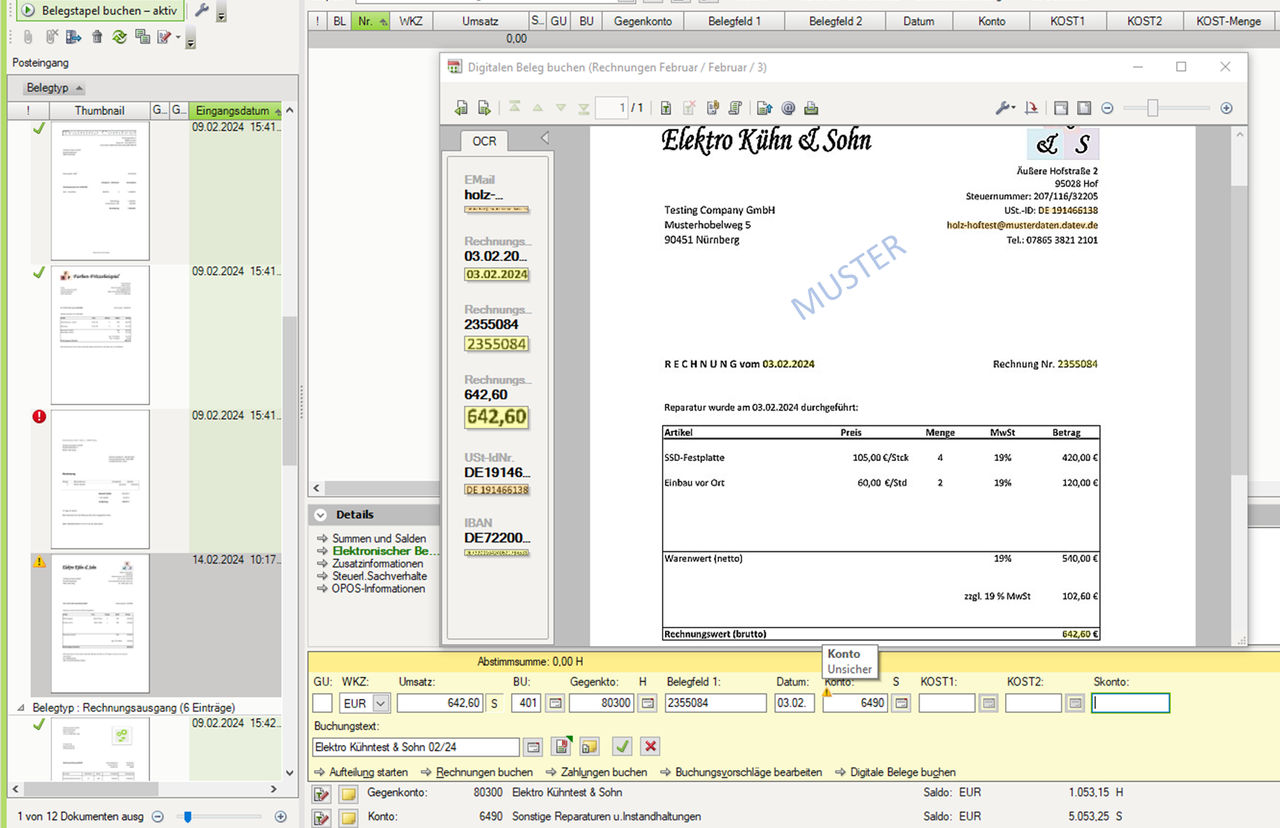
\includegraphics[width=0.7\textwidth]{images/datev-automatisierung-rechnungen}
        \end{center}
    \end{frame}

    \begin{frame}{Requirements}
        Performance by \emph{Neural AI}:
        \begin{itemize}
            \item Handle most cases without the need of human supervision
            \item Understand scenarios based on world knowledge (e.g. "Lindt" in a position indicates choclate consumption)
        \end{itemize}

        Trust and manipulations by \emph{Symbolic AI}:
        \begin{itemize}
            \item Customers need to guarantee certain behaviour, such as respectation of laws
            \item Manipulation of models based on human input
        \end{itemize}

        \begin{center}
            \bf This requires a form of neuro-symbolic AI!
        \end{center}
    \end{frame}

    \begin{frame}{Toy Accounting Example}
        To showcast the approach we study a toy accounting example.
        For each invoice three variables are either $\truesymbol$ or $\falsesymbol$:
        \begin{itemize}
            \item A $\var{Feature}$ is present on the receipt (e.g. whether the receipt was received or sent by the customer).
            \item The account $\var{Account 1}$ is used to book the receipt.
            \item The account $\var{Account 2}$ is used to book the receipt.
        \end{itemize}

        Let there be two accounting rules to be respected:
        \begin{itemize}
            \item Exactly one of the accounts $\var{Account 1}$ and $\var{Account 2}$ is used to book the receipt.
            \item When the $\var{Feature}$ is present on the receipt, the $\var{Account 1}$ needs to be booked.
        \end{itemize}
    \end{frame}

    \begin{frame}{Realistic Problem Sizes}
        The variables and main relations are visualized in a so-called ontology\footnote{\tiny https://github.com/EnexaProject/enexa-use-case-1-business-software-solutions}:
        \begin{center}
            \begin{tikzpicture}
                \drawtextnode{0}{0}{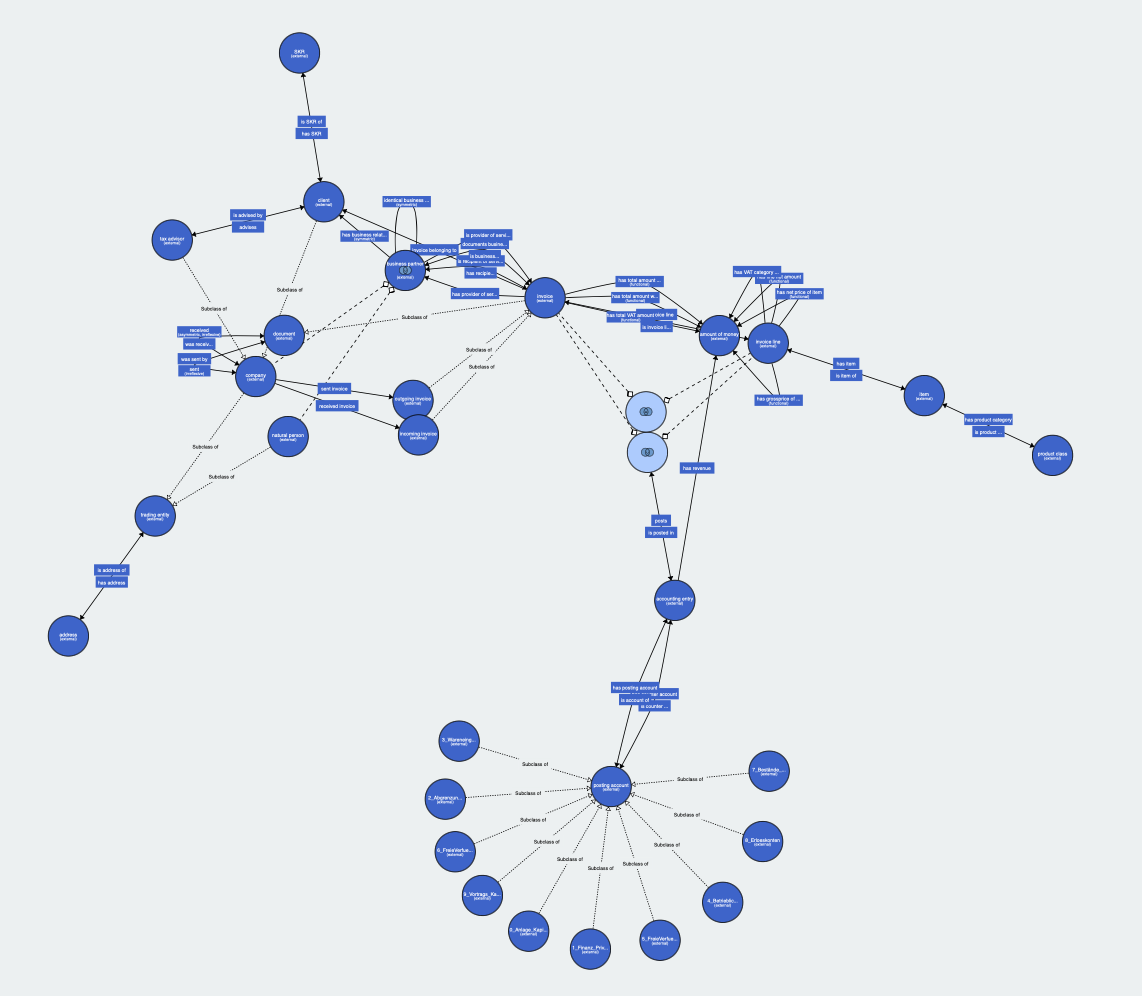
\includegraphics[height=0.4\textwidth]{images/ontology_fine_snapshot}}
                \drawtextnode{0}{-3}{\bf Coarse Visualization}
                \drawtextnode{5}{0}{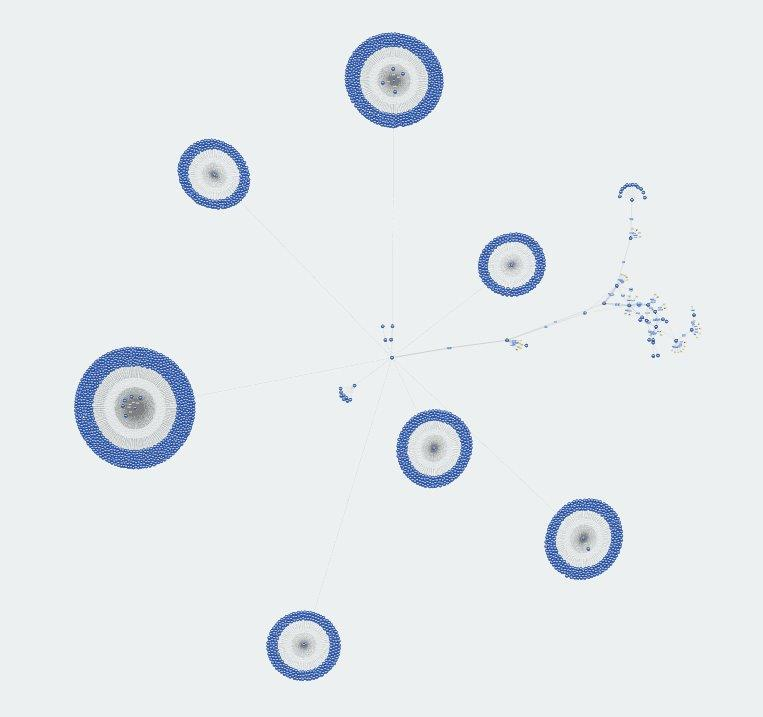
\includegraphics[height=0.4\textwidth]{images/ontology_coarse_snapshot}}
                \drawtextnode{5}{-3}{\bf Detailed Visualization}
            \end{tikzpicture}
        \end{center}
        \begin{center}
            We will come back to ontologies and knowledge graphs later in the course.
        \end{center}
    \end{frame}

    \section{Tensors in Artificial Intelligence}

    \begin{frame}{Representation of the toy accounting system}
        The system has a representation by the variables taking values in $\{0,1\}$ (i.e. $\catdim=2$):
        \begin{itemize}
            \item $\catvariableof{F}$: Whether the $\var{Feature}$ is present on the receipt.
            \item $\catvariableof{A1}$: Whether the  $\var{Account 1}$ is used.
            \item $\catvariableof{A2}$: Whether the  $\var{Account 2}$ is used.
        \end{itemize}

        The system states are the cartesian product of the variable states $\{0,1\}$:
        \begin{align*}
            \bigtimes_{\catenumerator\in\{F,A1,A2\}} \{0,1\}
            = \{&(0,0,0), (0,0,1), (0,1,0), (0,1,1), \\
            &(1,0,0), (1,0,1), (1,1,0), (1,1,1)\}
        \end{align*}
        The toy accounting rules exclude some states:
        \begin{itemize}
            \item Exactly one of the accounts $\var{Account 1}$ and $\var{Account 2}$ is used to book the receipt: $\catvariableof{F}\Rightarrow\catvariableof{A1}$
            \item When the $\var{Feature}$ is present on the receipt, the $\var{Account 1}$ needs to be booked: $\catvariableof{A1}\oplus\catvariableof{A2}$
        \end{itemize}
    \end{frame}

    \begin{frame}{Coordinatewise tensor visualization}
        Boolean tensors of leg-dimension $\catdim=2$ are
        \begin{align*}
            \hypercore \defcols \bigtimes_{\catenumerator\in\{0,\ldots,\catorder-1\}} \{0,1\} \rightarrow \rr \, .
        \end{align*}
        We visualize such maps as
        \begin{itemize}
            \item \textbf{$\catorder=1$: Vectors}
            \begin{align*}
                \catvariableof{A1}: \quad
                \begin{pmatrix}
                    0 \\ 1
                \end{pmatrix}
            \end{align*}
            \item \textbf{$\catorder=2$: Matrices}
            \begin{align*}
                \catvariableof{A1}\oplus\catvariableof{A2}: \quad
                \begin{pmatrix}
                    0 & 1 \\ 1 & 0
                \end{pmatrix}
                \quad, \quad
                \catvariableof{F}\Rightarrow\catvariableof{A1}: \quad
                \begin{pmatrix}
                    1 & 1 \\ 0 & 1
                \end{pmatrix}
            \end{align*}
            \item \textbf{$\catorder=3$: Order-3 tensors}
            \begin{center}
                \begin{tikzpicture}[scale=1]
                    \drawtextnode{-3}{0.25}{$(\catvariableof{A1}\oplus\catvariableof{A2})\land(\catvariableof{F}\Rightarrow\catvariableof{A1})$:}
                    \node (A) at (0,0) {
                        $\begin{pmatrix}
                             0 & 1 \\ 1 & 0
                        \end{pmatrix}$
                    };
                    \node at (1.25,0.5){
                        $\begin{pmatrix}
                             0 & 0 \\ 1 & 0
                        \end{pmatrix}$
                    };
                \end{tikzpicture}
            \end{center}
        \end{itemize}
    \end{frame}

    \begin{frame}{Tensors: Natural description of factored representations}
    {\bf Factored representations}
        are collection of variables $\{\catvariableof{0},\ldots,\catvariableof{\catorder-1}\}$, each with a finite set of states $\{0,\ldots,\catdimof{\catenumerator}-1\}$ (so far: $\{0,1\}$ for $\catdim=2$).
        The set of states is then the cartesian product
        \begin{align*}
            \bigtimes_{\catenumerator\in\{0,\ldots,\catorder-1\}} \{0,\ldots,\catdimof{\catenumerator}-1\}
        \end{align*}

            {\bf Knowledge about the system}, for example the possibility of each state, is a \emph{tensor}
        \begin{align*}
            \hypercore \defcols \bigtimes_{\catenumerator\in\{0,\ldots,\catorder-1\}} \{0,\ldots,\catdimof{\catenumerator}-1\} \rightarrow \rr
        \end{align*}
    \end{frame}

    \begin{frame}{Tensors for neuro-symbolic AI}
        Tensors (and their networks) are a unifying language for Artificial Intelligence
        \begin{itemize}
            \item {\bf Logical knowledge bases:} Boolean coordinates, decomposition by logical syntax
            \item {\bf Probability distributions:} Non-negative coordinates, decomposition by independencies
            \item {\bf Neural networks:} Representation of arbitrary function decompositions
            \item {\bf Data bases:} Relations stored in tables are tensors
        \end{itemize}

        Tensors capture the
        \begin{itemize}
            \item \emph{Structure of symbolic AI}
            \item \emph{Flexibility of neural AI}
        \end{itemize}

        \begin{center}
            \bf We exploit the tensor formalism in this course for neuro-symbolic AI.
        \end{center}
    \end{frame}

    \begin{frame}{Tensors for neuro-symbolic AI}
        \begin{itemize}
            \item {\bf Modelling principle:}
            Representation of logical and probabilistic models by tensors.
            \item {\bf Sparsity principle:}
            Decomposition of tensors into tensor networks.
            \item {\bf Inference principle:}
            Contractions of tensor networks.
        \end{itemize}

        The course orients on the preprint:
        \begin{center}
            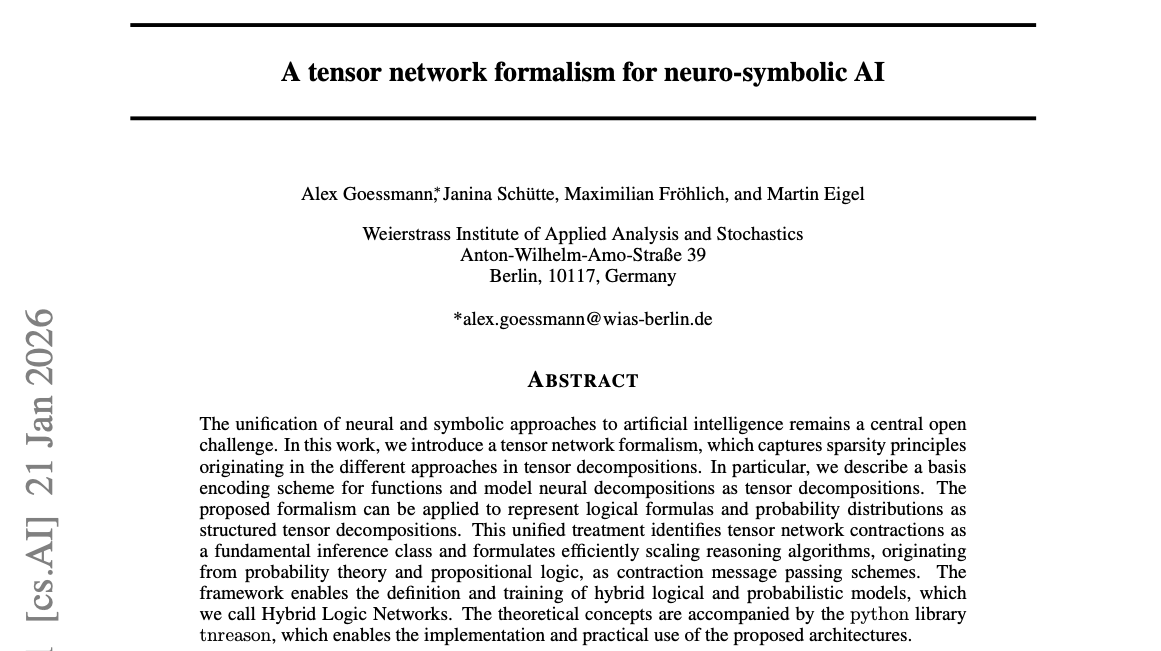
\includegraphics[width=0.7\textwidth]{images/arxiv_snap}
        \end{center}
    \end{frame}

    \begin{frame}{Tensors:
    A computational interface for Machine Learning}

        On the \emph{software} side:
        \begin{itemize}
            \item Parallel computing enabled through (multi-)linear algebra
            \item Tensors are main classes is standard ML libraries: TensorFlow, Pytorch
        \end{itemize}

        On the \emph{hardware} side:
        \begin{itemize}
            \item Dedicated for graphic processing: Graphic Processing Units (GPUs)
            \item AI-dedicated hardware: Tensor Processing Units (TPUs)
        \end{itemize}
        \begin{center}
            
\includegraphics[width=0.5\textwidth]{images/tensorflow.png}
            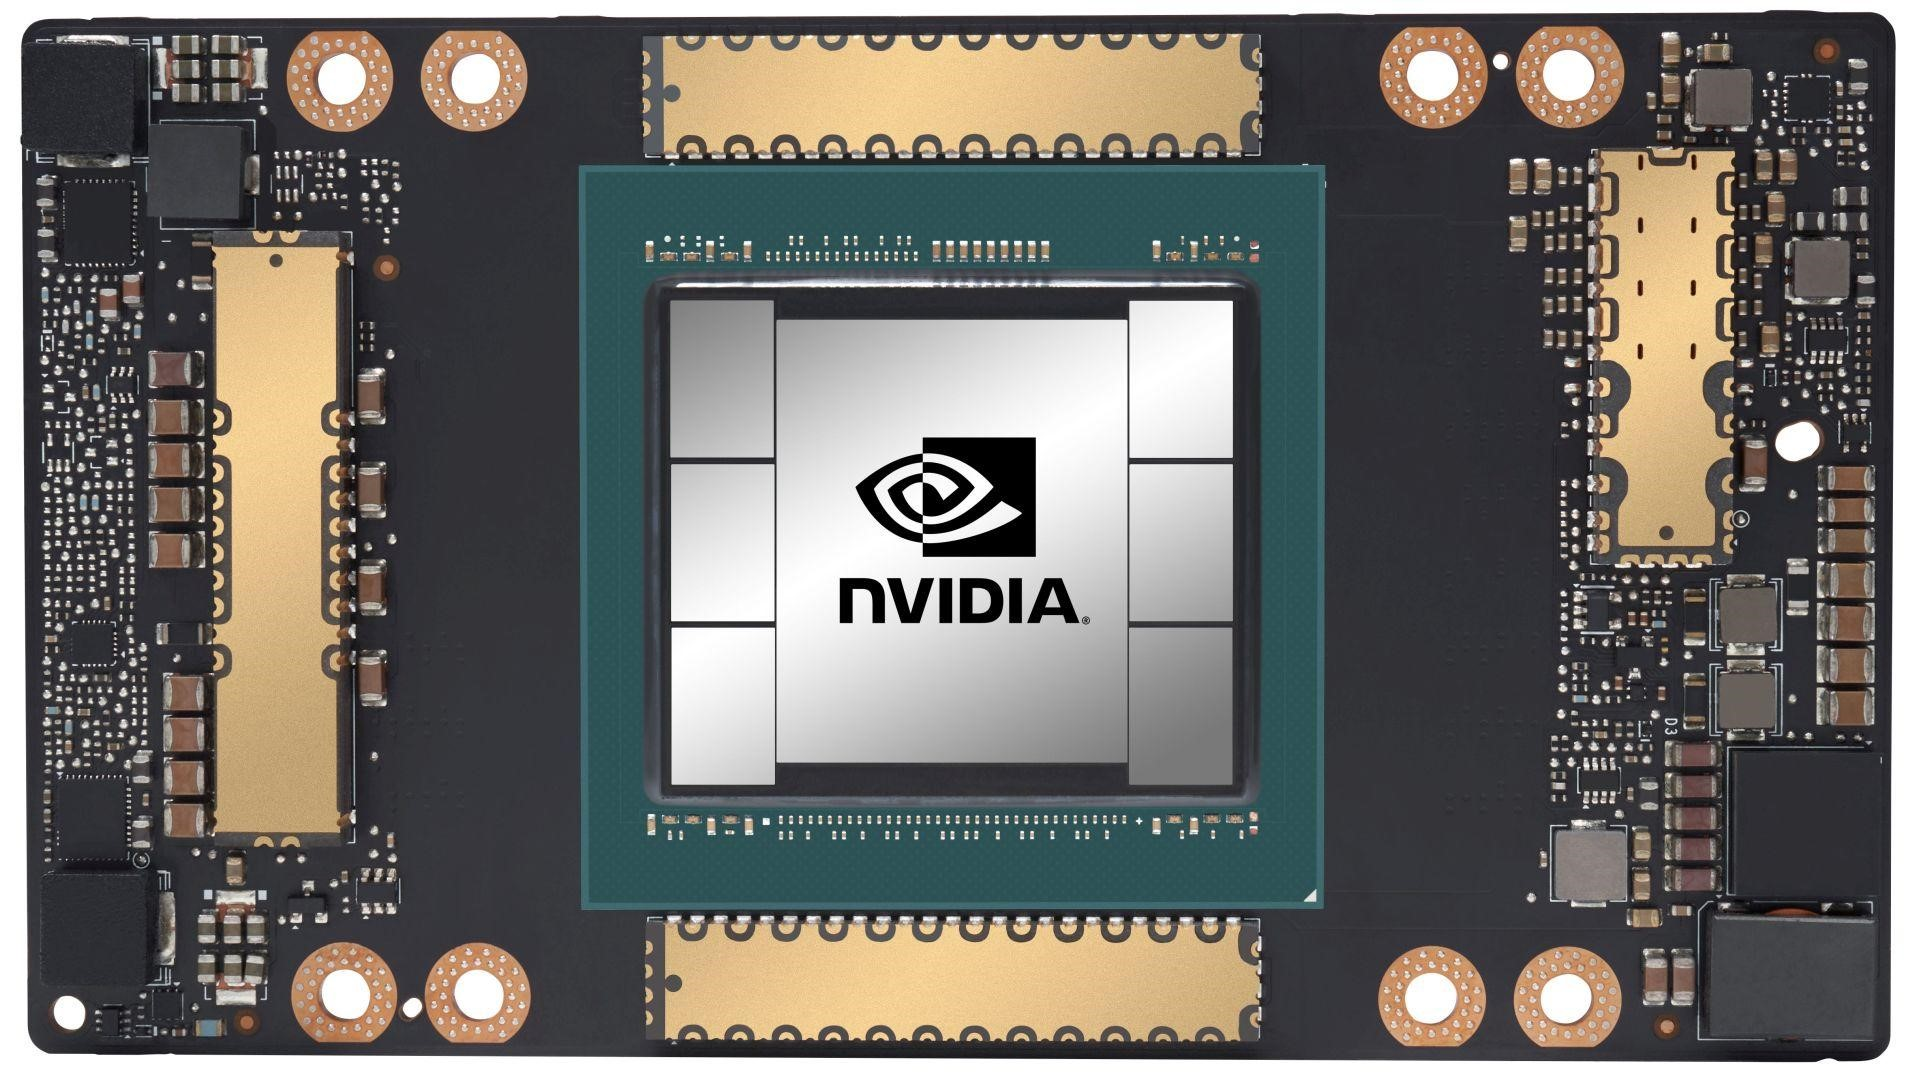
\includegraphics[width=0.2\textwidth]{images/nvidia-a100.jpeg}
            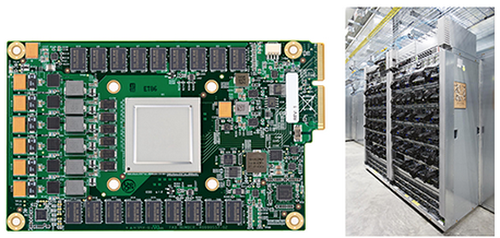
\includegraphics[width=0.3\textwidth]{images/google_tpu.png}
        \end{center}
    \end{frame}

    \section{Topics of the course}

    \begin{frame}{I - Logical Approaches}
        \begin{minipage}{0.65\linewidth}
            Logic as the theory of human reasoning:
            \begin{itemize}
                \item Dating back to greek philosophers modelling Human Intelligence
                \item Traditional approaches to Artificial Intelligence
            \end{itemize}

            Logics consists in
            \begin{itemize}
                \item {\bf Syntax:} Description of knowledge
                \item {\bf Semantics:} Interpretation of knowledge, inference of new knowledge
            \end{itemize}
            \begin{block}{Challenges}
                \begin{itemize}
                    \item Find sparse representation mechanisms
                    \item Efficient reasoning schemes based on tensor network contractions
                \end{itemize}
            \end{block}
        \end{minipage}
        \begin{minipage}{0.3\linewidth}
            \begin{center}
                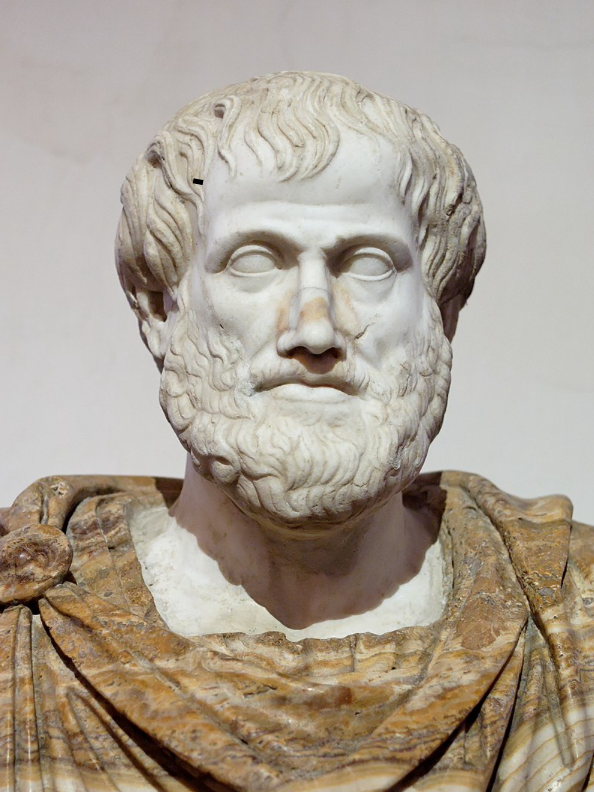
\includegraphics[width=2cm]{images/aristotle.png}\\
                {\tiny Aristotle}\footnote{\tiny https://de.wikipedia.org/wiki/Aristoteles} \\
                \medskip
                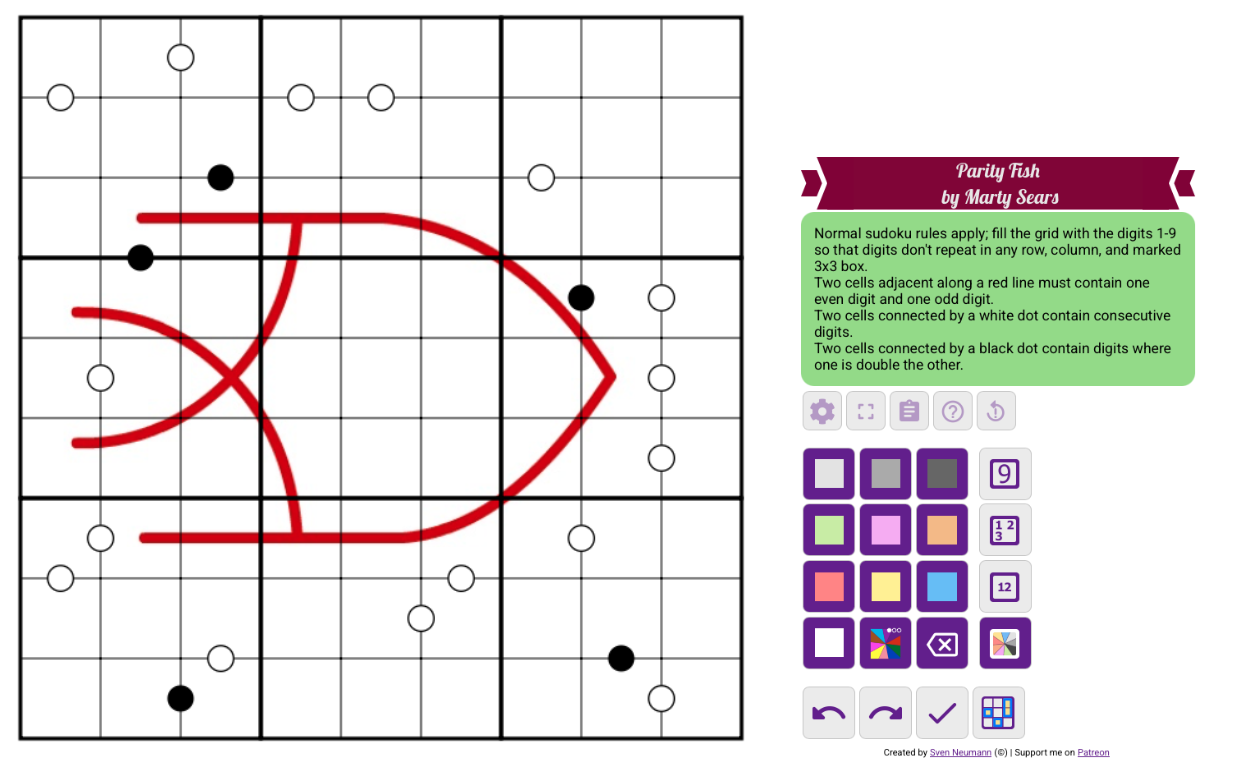
\includegraphics[width=3cm]{images/sakana_fish.png}\\
                {\tiny Modified Sudoku puzzles}\footnote{\tiny https://sakana.ai/sudoku-bench/} \\
            \end{center}
        \end{minipage}
    \end{frame}

    \begin{frame}{II - Probabilistic Approaches}
        Bayesian Networks model probabilistic relations between variables
        \begin{center}
            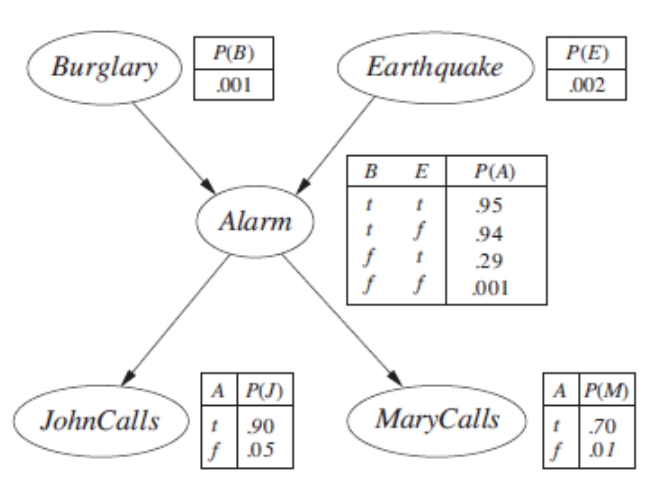
\includegraphics[width=6cm]{images/burglary.png}
        \end{center}

        \begin{block}{Challenges}
            \begin{itemize}
                \item Learn the dependence structure of the variables
                \item Extract the causal relations of the variables
            \end{itemize}
        \end{block}
    \end{frame}

    \begin{frame}{III - Statistical Models of Knowledge Graphs}
        Extension from factored representations to \emph{structured representations}:
        \begin{itemize}
            \item Worlds contain objects from classes.
            \item The objects are enumerated using further tensor axes.
        \end{itemize}
        \begin{center}
            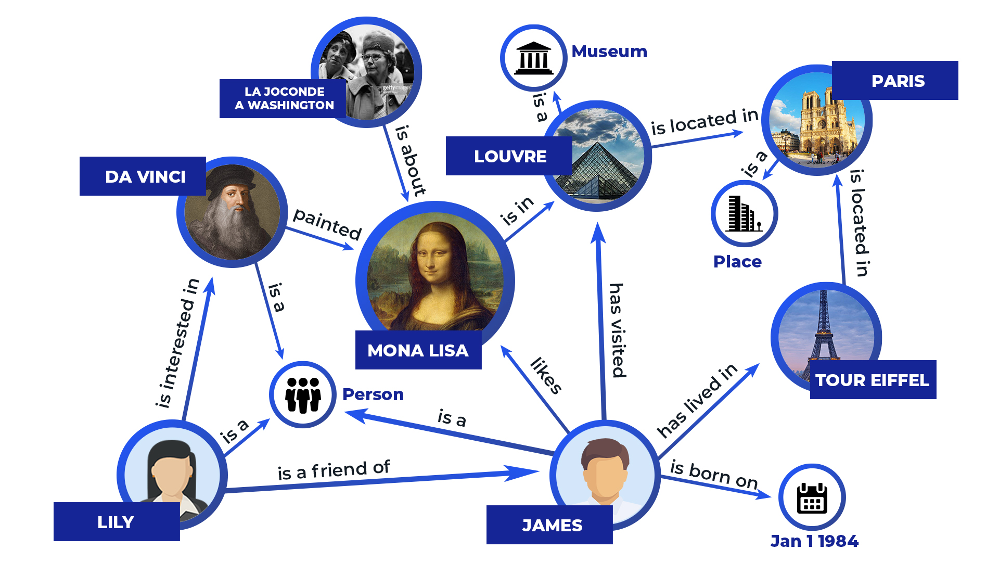
\includegraphics[width=0.6\textwidth]{images/kg-example.png}\footnote{\tiny https://ml-digest.com/knowledge-graphs/}
        \end{center}
        \begin{block}{Challenges}
            \begin{itemize}
                \item Reason about the relations in a knowledge graph
                \item Predict the connectivity of new objects
            \end{itemize}
        \end{block}
    \end{frame}

    \begin{frame}{IV - Quantum Machine Learning}
        \begin{minipage}{0.55\linewidth}
            Quantum computation
            \begin{itemize}
                \item Formulated in tensor spaces
                \item Quantum circuits: Tensor networks
            \end{itemize}
            Quantum machine learning
            \begin{itemize}
                \item Inference in quantum circuits
                \item Promise: Efficiency increase (to be shown)
            \end{itemize}
        \end{minipage}
        \begin{minipage}{0.4\linewidth}
            \begin{center}
                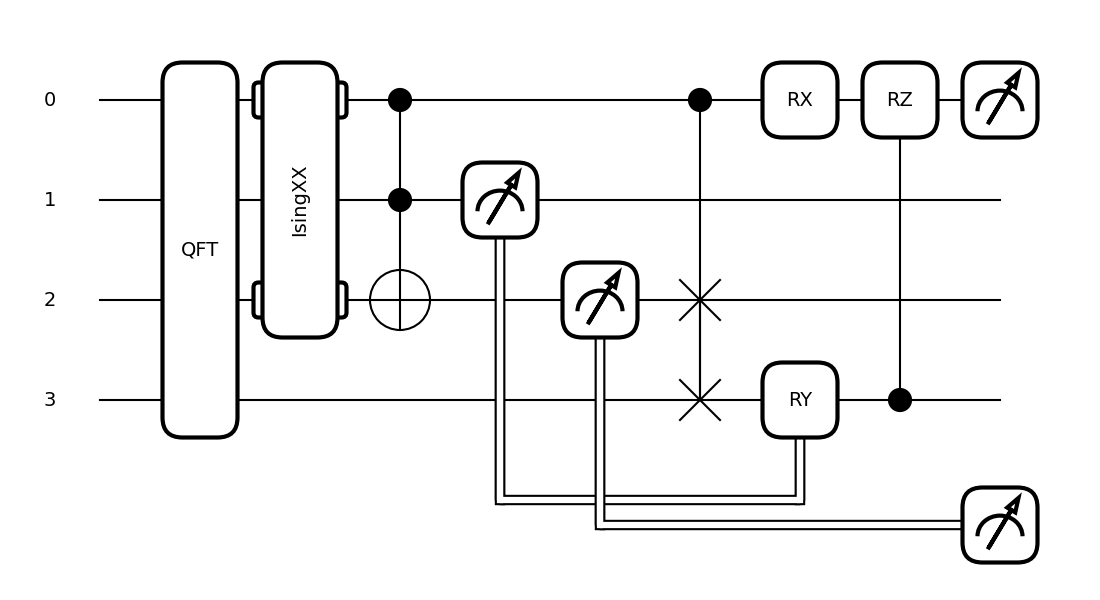
\includegraphics[width=1\textwidth]{images/circuit-example.png} \\
                {\tiny Example of a Quantum Circuit\footnote{\tiny https://docs.pennylane.ai/en/stable/introduction/inspecting-circuits.html}:}
            \end{center}
        \end{minipage}

        \begin{block}{Challenges}
            \begin{itemize}
                \item Find sparse quantum circuits exploiting a models sparsity
                \item Increase the efficiency of reasoning with tensor networks by quantum computation.
            \end{itemize}
        \end{block}
    \end{frame}

    \begin{frame}{Further literature}
        Introductory textbooks:
        \begin{itemize}
            \item \textbf{Russel, Norvig: Artificial Intelligence - A Modern Approach} (Fourth Edition), Pearson Education 2021
            \item \textbf{Koller, Friedman: Probabilistic Graphical Models: Principles and Techniques}, MIT Press 2009
            \item \textbf{Antoniou et al: A Semantic Web Primer} (Third Edition), MIT 2012
            \item \textbf{Schuld, Petruccione: Machine Learning with Quantum Computers}, Springer 2021
        \end{itemize}

        Advanced textbooks:
        \begin{itemize}
            \item \textbf{Wainwright, Jordan: Graphical Models, Exponential Families and Variational Inference}, now 2008
            \item \textbf{Hackbusch: Tensor Spaces and Numerical Tensor Calculus}, Springer 2019
        \end{itemize}
    \end{frame}

\end{document}